\chapter{4-methoxy-pyridine complexes}
\section{\ce{[Co(N_3)_2(4-methoxypyridine)_4]}}
\label{CoA4MOP}
\subsection{Synthesis}
0.28 g \ce{CoSO_4 * 7 H_2O} (1 mmol), 0.13 g sodium azide (2 mmol) and 0.44 g 4-methoxy-pyridine (4 mmol) were dissolved in 20 mL distilled water. The solution was warmed up to $60^\circ$C  and stirred for 2 hours and 30 minutes. The clear pink solution was stirred again after filtration for 1 hour at the same temperature and then cooled down to 20$^\circ$C. Pink crystals were obtained after one day.\\ Anal. Calculated for \ce{C_{24}H_{28}CoN_{10}O_{4}} (579.49 g/mol) : 49.74\% C; 4.87\% H; 24.17\% N;\\
Found: 49.45 \% C; 4.84\% H; 24.32 \% N;\\
IR (ATR, cm$^{-1}$): 2037 (m), 1603 (s), 1564 (m), 1508(m), 1495 (m),1454 (m), 1430 (m), 1291 (s), 1207 (s), 1057 (w), 1020 (s), 805 (s), 642 (w), 539 (s), 457 (w)

\begin{figure}[h!]
\centering
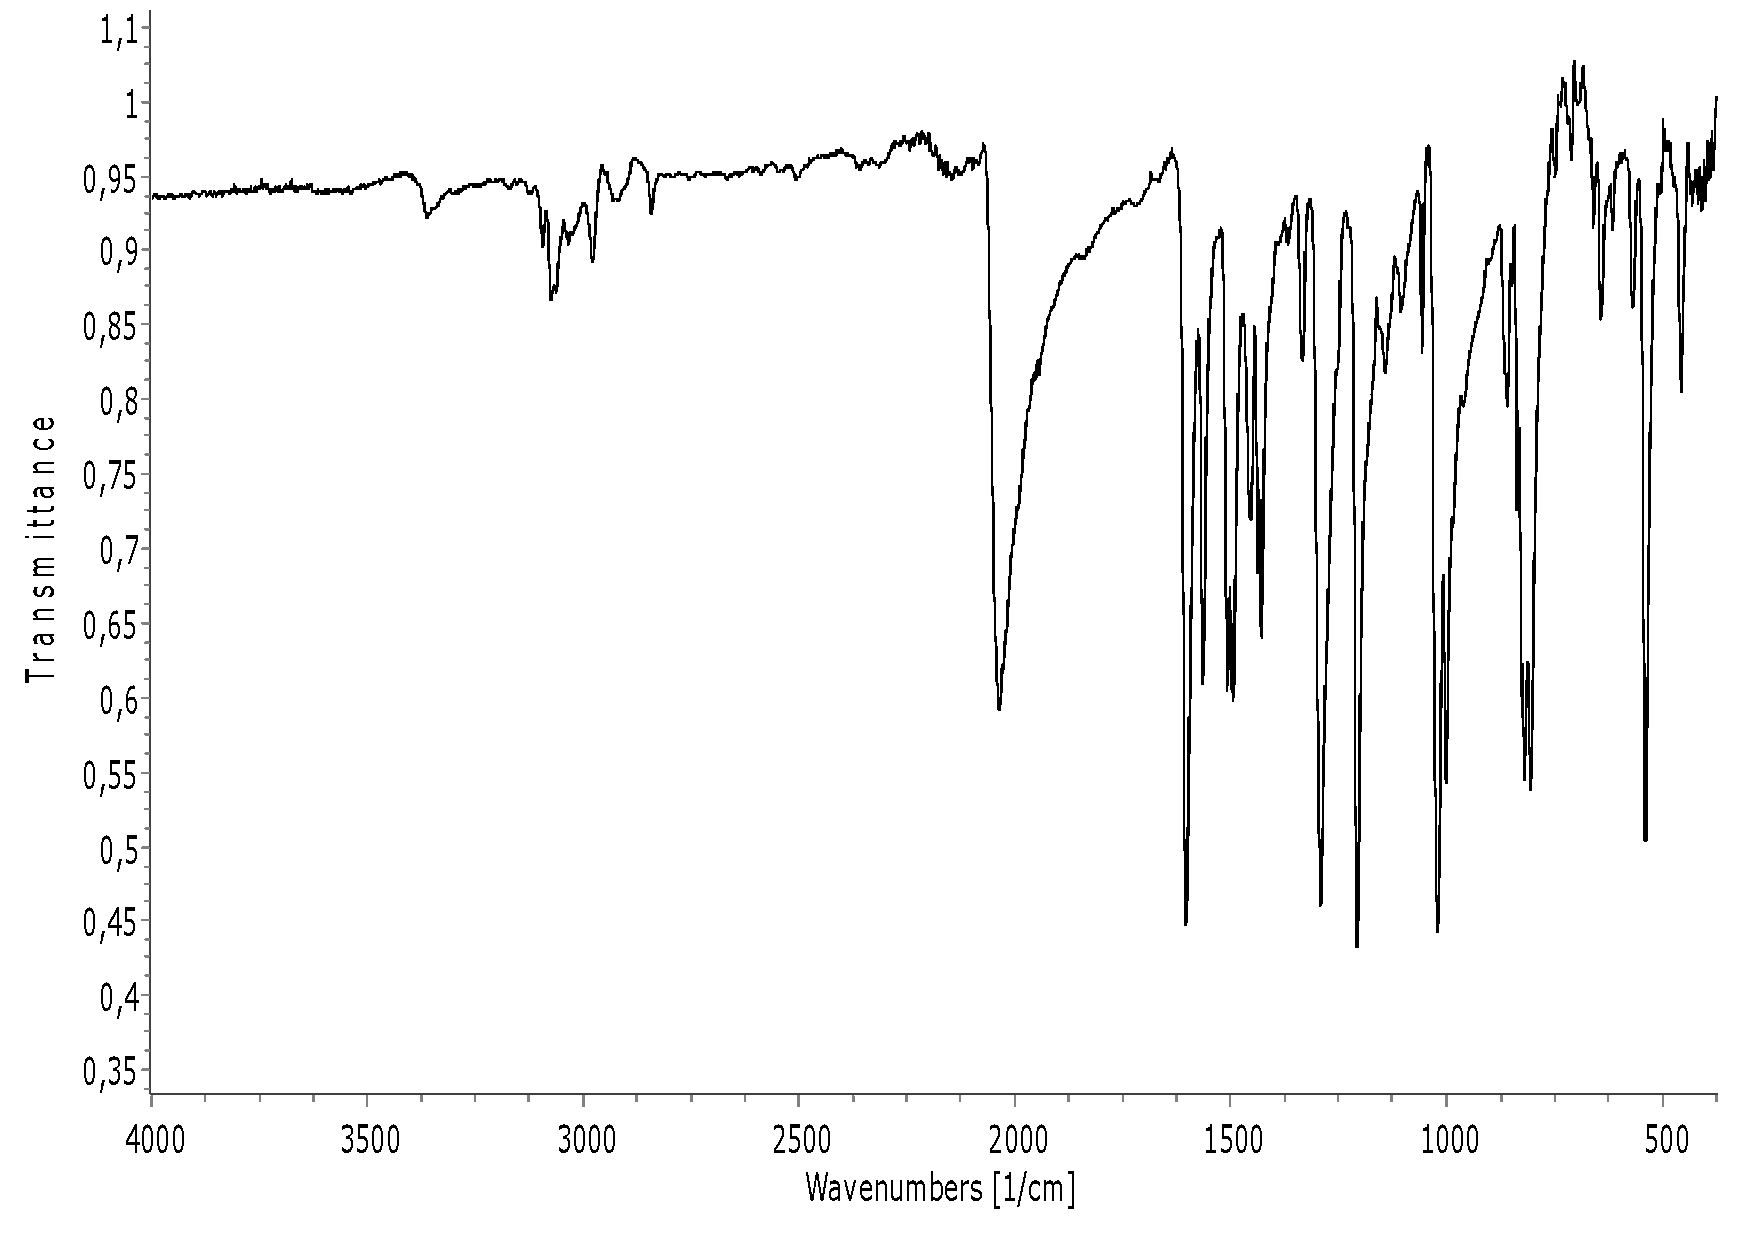
\includegraphics[scale=0.5, width=0.95\textwidth]{figures/CoA4MOP-IR.pdf}
\caption{IR spectrum of \ce{[Co(N_3)_2(4-MeOpy)_4]}}
\end{figure}

\newpage
\subsection{Structural characterization}

Fig. \ref{fig:CoA4MOP_pv} and fig. \ref{fig:CoA4MOP_packv} show a perspective view and a packing view of  \ce{[Co(N_3)_2(4-MeOpy)_4]}. Selected bond parameters are summarized in table \ref{batlb:CoA4MOP}. The complex consists of two crystallographically independent mononuclear and neutral Co(II) complexes. Each Co(II) is six-coordinated by N atoms of two terminal azido groups, as well as N-donor atoms of four neutral 4-methoxy-pyridine molecules. The \ce{CoN_6} chromophores may be described as slighly distorted octahedra with trans-arrangement of the azido ligands. The Co-N bond lengths are in the range of 2.085(3) to 2.202(3) \AA , and the transoid N-Co-N bond angles within the \ce{CoN_6} octahedra vary from 171.61(11) to 177.35(12)$^\circ$. The bond parameters of the terminal azido groups are: Co-N-N: from 125.6(2) to 129.1(3)$^\circ$, N-N-N: from 178.3(4) to 179.3(4)$^\circ$, N(x1)-N(x2): from 1.192(4) to 1.199(4) \AA, N(x2)-N(x3): from 1.165(5) to 1.175(4) \AA.The shortest metal-metal separation is 8.2523(8) \AA. 


\renewcommand{\arraystretch}{1.5}
\begin{table}
\captionabove{Selected bond lengths (\AA) and angles ($^\circ$) for  \ce{[Co(N_3)_2(4-MeOpy)_4]}}
\centering
\begin{tabular}{|l|l|l|l|}
\hline
Co(1)-N(11) & 2.103(3) & Co(2)-N(31) & 2.116(3)\\
\hline
Co(1)-N(21) & 2.125(3) & Co(2)-N(41) & 2.085(3)\\
\hline
Co(1)-N(1) & 2.170(3) & Co(2)-N(5) & 2.173(3)\\
\hline
Co(1)-N(2) & 2.184(3) & Co(2)-N(6) & 2.181(3)\\
\hline
Co(1)-N(3) & 2.189(3) & Co(2)-N(7) & 2.202(3)\\
\hline
Co(1)-N(4) & 2.161(3) & Co(2)-N(8) & 2.188(3)\\
\hline
N(11)-N(12) & 1.196(4) & N(12)-N(13) & 1.167(4)\\
\hline
N(21)-N(22) & 1.194(4) & N(22)-N(23) & 1.175(4)\\
\hline
N(31)-N(32) & 1.192(4) & N(32)-N(33) & 1.167(5)\\
\hline
N(41)-N(42) & 1.199(4) & N(42)-N(43) & 1.165(5)\\
\hline
\hline
N(11)-Co(1)-N(21) & 176.97(12) & N(31)-Co(2)-N(41) & 177.35(12)\\
\hline
N(1)-Co(1)-N(3) & 175.60(11) & N(5)-Co(2)-N(8) & 171.61(11)\\
\hline
N(2)-Co(1)-N(4) & 174.15(11) & N(6)-Co(2)-N(7) & 175.88(11)\\
\hline
Co(1)-N(11)-N(12) & 125.6(2) & N(11)-N(12)-N(13) & 178.7(4)\\
\hline
Co(1)-N(21)-N(22) & 128.2(2) & N(21)-N(22)-N(23) & 178.3(4)\\
\hline
Co(2)-N(3)-N(32) & 129.1(3) & N(31)-N(32)-N(33) & 179.3(4)\\
\hline
Co(2)-N(41)-N(42) & 126.0(3) & N(41)-N(42)-N(43) & 178.6(4)\\
\hline
\end{tabular}
\label{batlb:CoA4MOP}
\end{table}













\begin{figure}[!htpb]
\centering
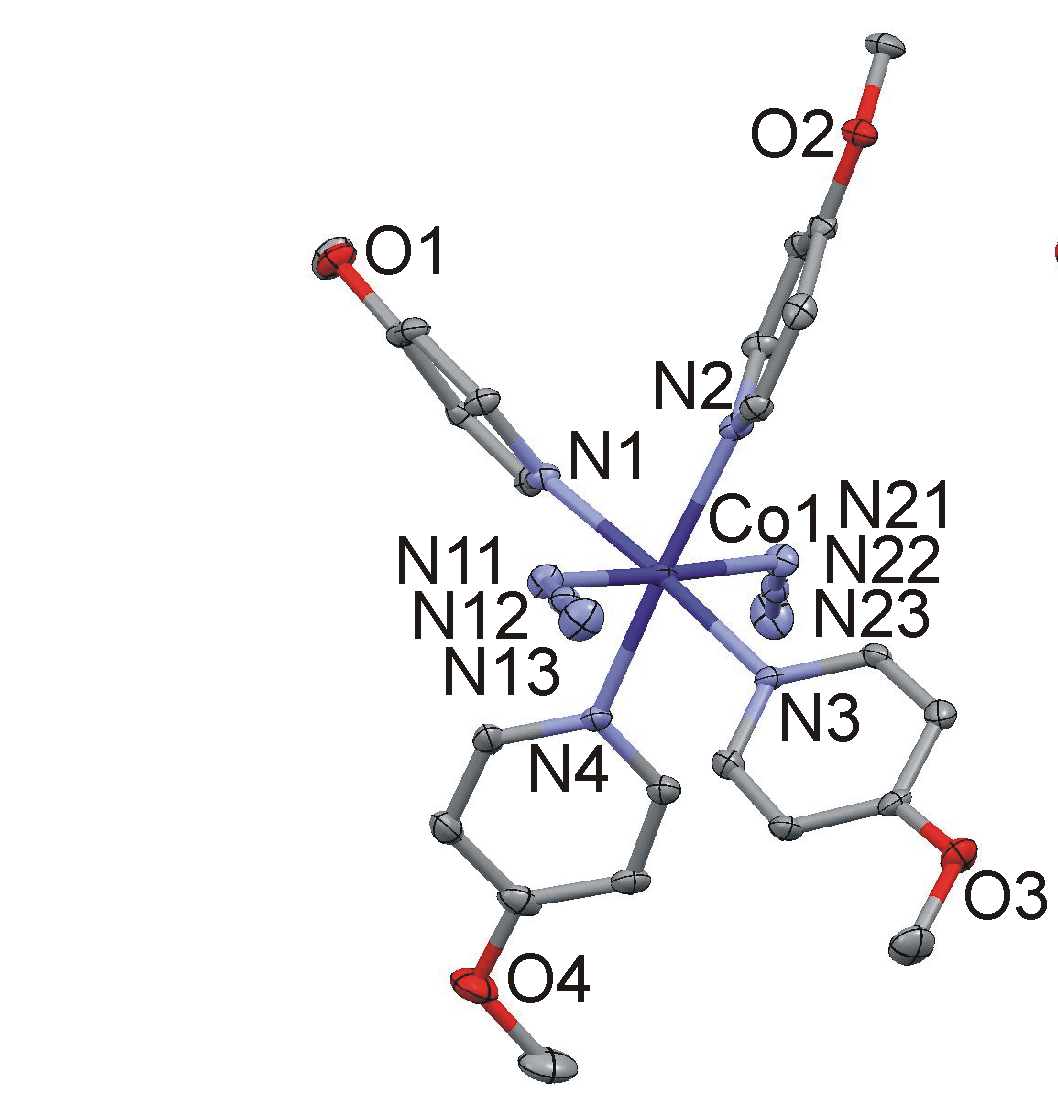
\includegraphics[width=1\textwidth]{figures/CO_4MOP_FIGm11.png}
\caption[Perspective view of \ce{[Co(N_3)_2(4-MeOpy)_4]}]{Perspective view of \ce{[Co(N_3)_2(4-MeOpy)_4]} with the atom numbering scheme.}
\label{fig:CoA4MOP_pv}
\vspace{\floatsep}
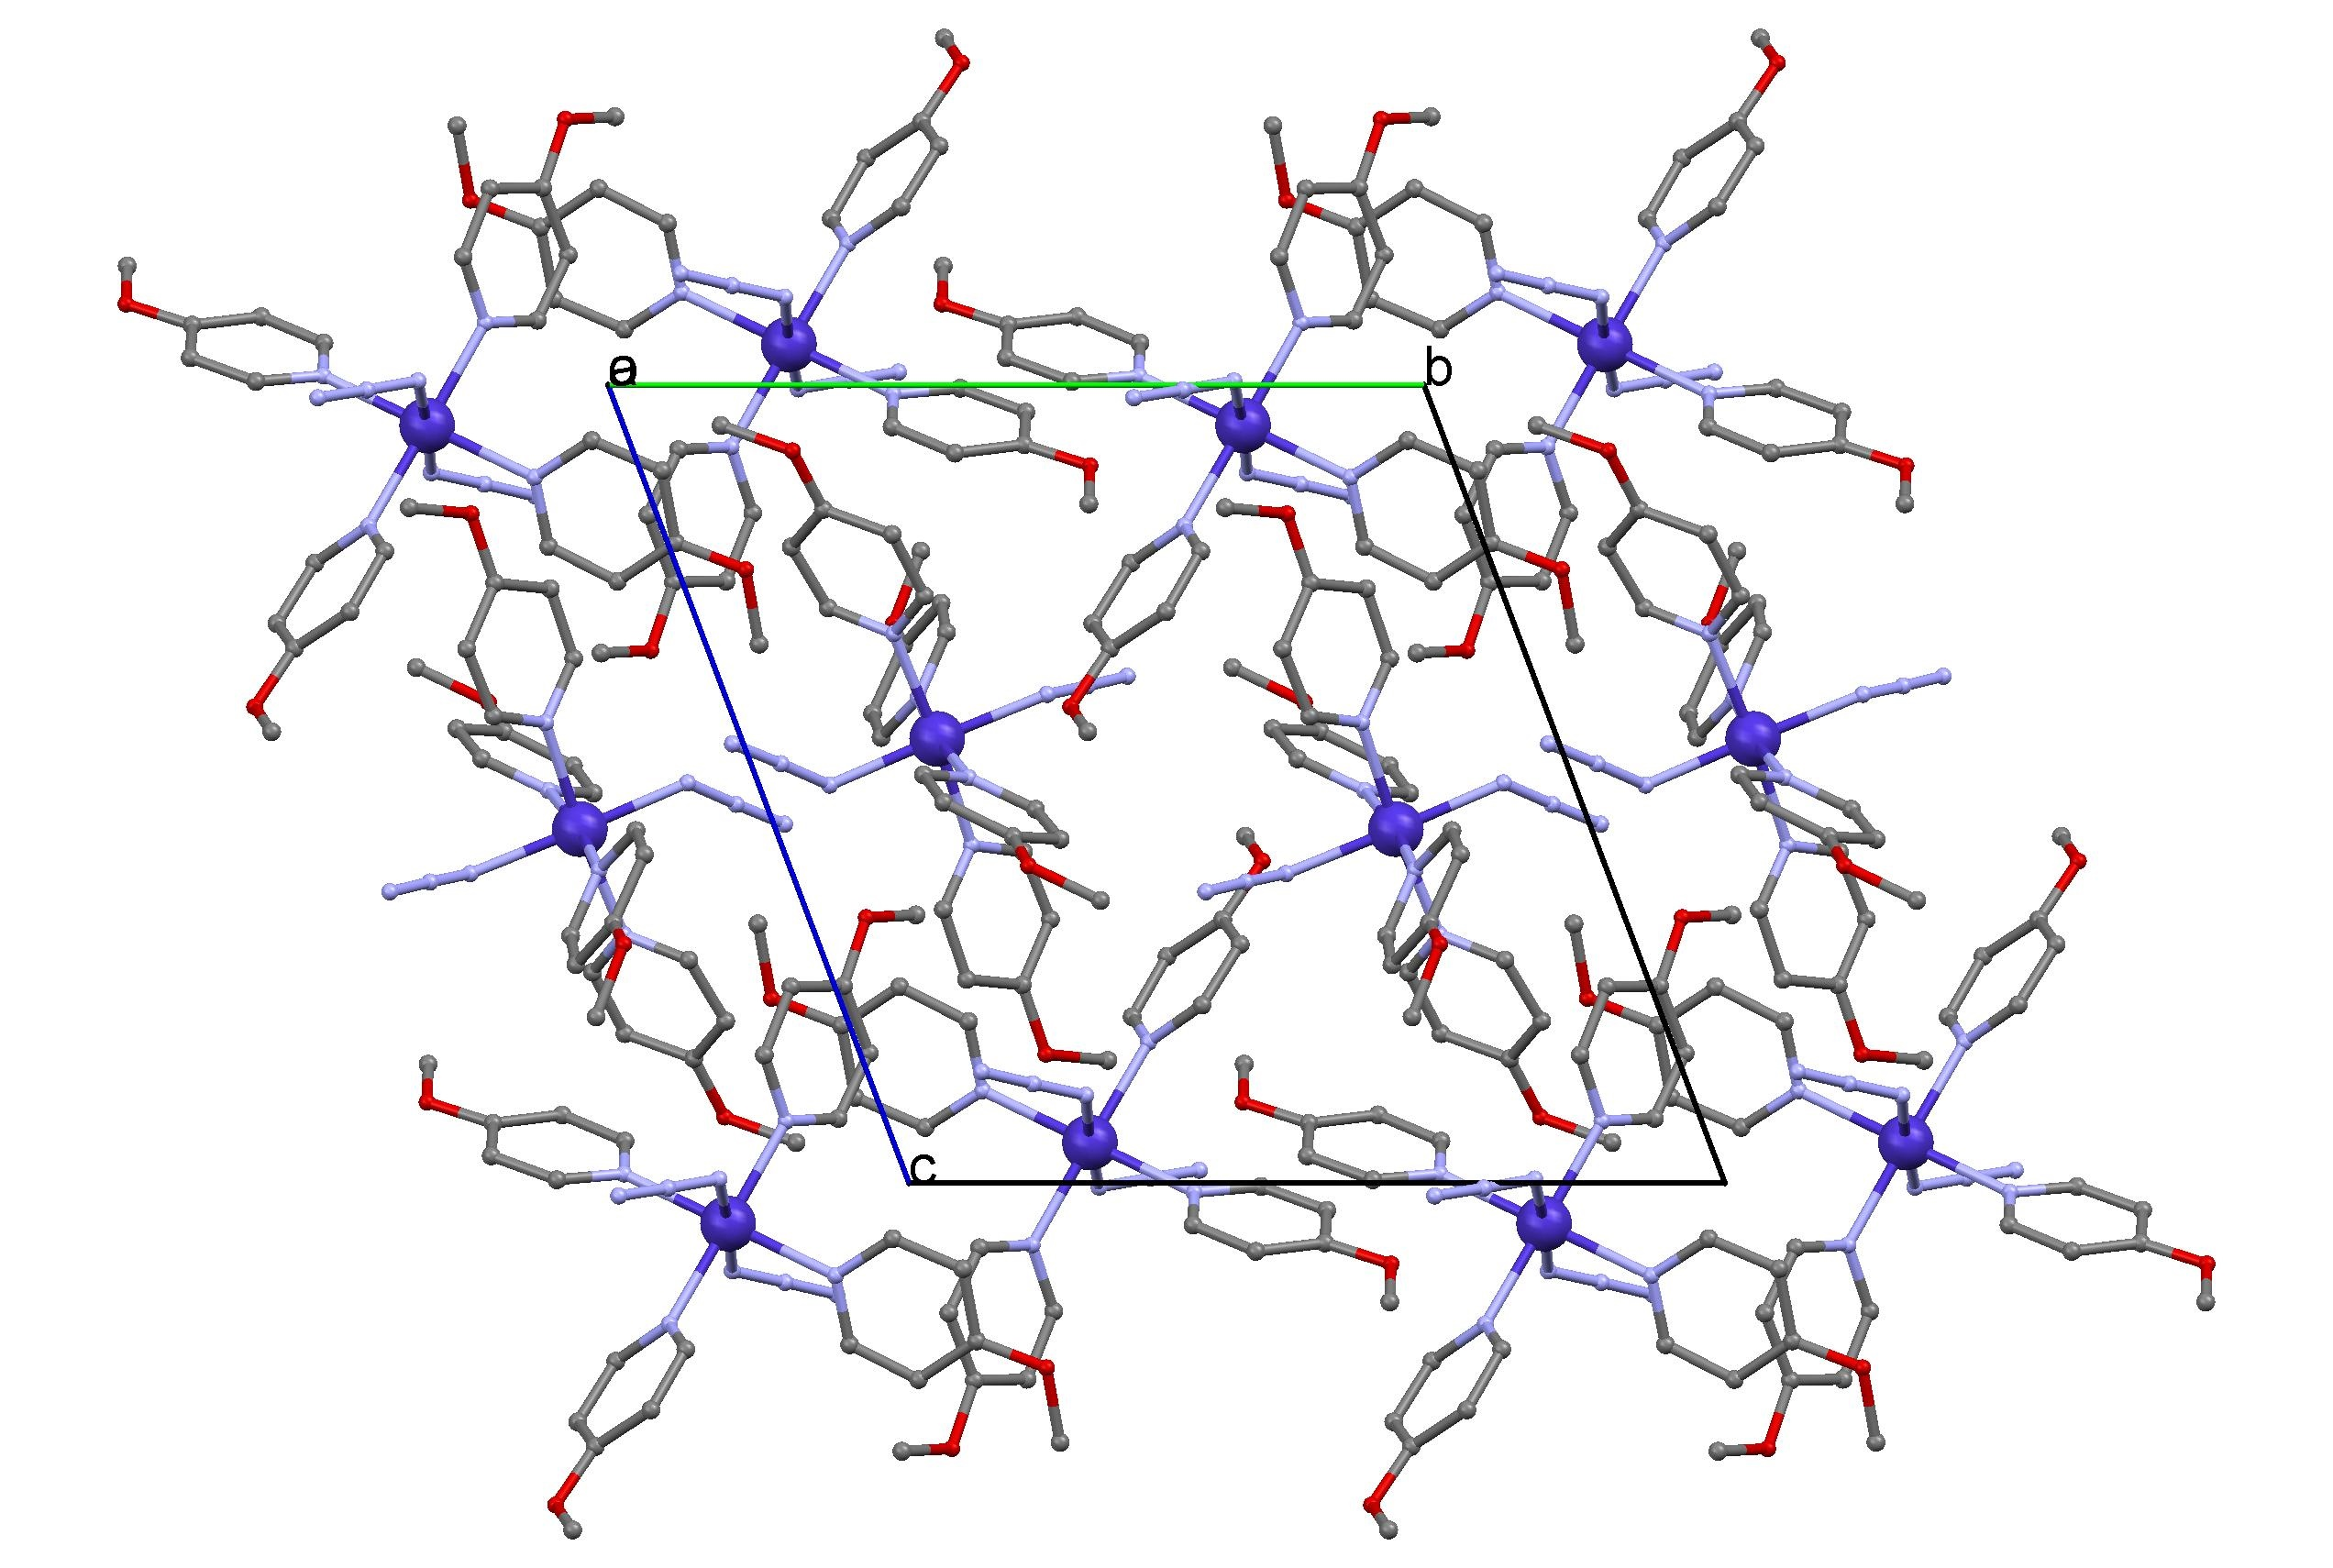
\includegraphics[width=1\textwidth]{figures/co_4mop_CA.jpg}
\caption{Packing view of \ce{[Co(N_3)_2(4-MeOpy)_4]}.}
\label{fig:CoA4MOP_packv}
\end{figure}




\begin{table}
\centering
\captionabove{Crystallographic data and processing parameter of \ce{[Co(N_3)_2(4-MeOpy)_4]}}
\begin{tabular}{ | l |  l | }
\hline
Empirical formula & \ce{C_{24}H_{28}CoN_{10}O_{4}}\\
\hline
Formula mass & 579.49\\
\hline
System & triclinic\\
\hline
Space group & P-1\\
\hline
a ({\AA}) & 12.7449(5)\\
\hline
b ({\AA}) & 14.6263(6)\\
\hline
c ({\AA}) & 16.4750(6)\\
\hline
$\alpha$ ($^\circ$) & 70.309(2)\\
\hline
$\beta$ ($^\circ$) & 68.118(2)\\
\hline
$\gamma$ ($^\circ$) & 88.507(2)\\
\hline
V (\AA$^{3}) $  & 2665.58(19)\\
\hline
Z & 4\\
\hline
T (K) & 100(2)\\
\hline
$\mu$ (mm$^{-1}$) & 0.695\\
\hline
 D$_{calc}$ (Mg/m$^{3}$) & 1.444\\
\hline
Crystal size (mm) & 0.23 x 0.17 x 0.10\\
\hline
$\theta$ max ($^\circ$) & 28.05\\
\hline
Data collected & 12857\\
\hline
Unique refl./ R$_{int}$ & 12857 / -----\\
\hline
Parameters & 712\\
\hline
Goodness-of-Fit on F$^{2}$ & 1.058\\
\hline
R1 / wR2 (all data) & 0.0608 /0.1495\\
\hline
Residual extrema (e/\AA$^{3}$) & 0.75 /-1.27\\
\hline
\end{tabular}
\label{ptbl:CoA4MOP}
\end{table}




